\documentclass{article}
\usepackage{tikz}
\usetikzlibrary{arrows.meta,positioning,calc,shapes.geometric}
\pagestyle{empty}
\begin{document}
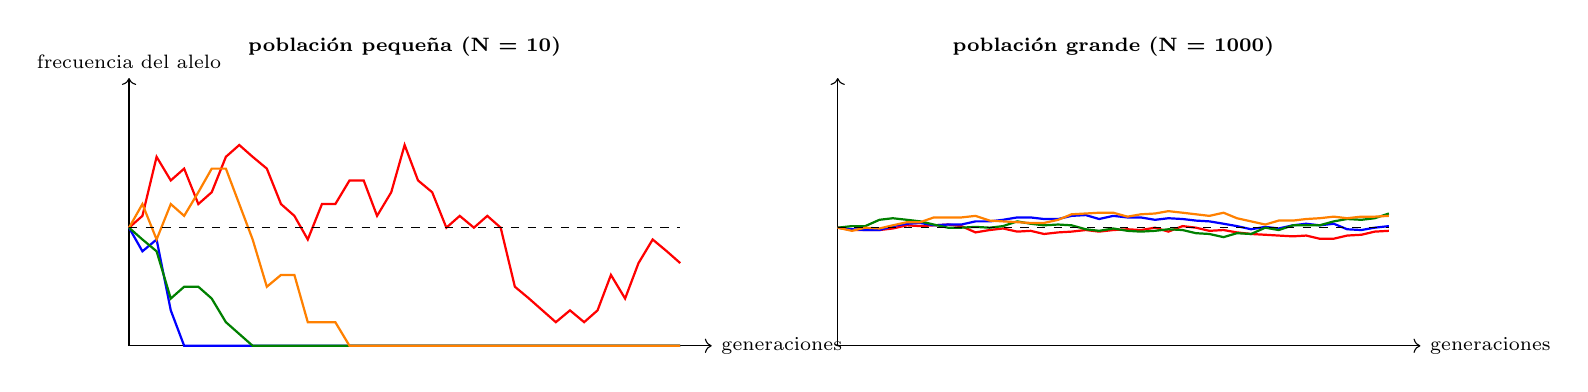
\begin{tikzpicture}
\draw[->] (0,0) -- (0,3.4) node[above, font=\scriptsize] {frecuencia del alelo}; \draw[->] (0,0) -- (7.4,0) node[right, font=\scriptsize] {generaciones}; \node[font=\bfseries\scriptsize] at (3.5,3.8) {población pequeña (N = 10)};
\draw[thick, red] plot coordinates {(0.00,1.50) (0.17,1.65) (0.35,2.40) (0.53,2.10) (0.70,2.25) (0.88,1.80) (1.05,1.95) (1.23,2.40) (1.40,2.55) (1.57,2.40) (1.75,2.25) (1.93,1.80) (2.10,1.65) (2.27,1.35) (2.45,1.80) (2.62,1.80) (2.80,2.10) (2.98,2.10) (3.15,1.65) (3.33,1.95) (3.50,2.55) (3.67,2.10) (3.85,1.95) (4.03,1.50) (4.20,1.65) (4.38,1.50) (4.55,1.65) (4.72,1.50) (4.90,0.75) (5.08,0.60) (5.25,0.45) (5.42,0.30) (5.60,0.45) (5.78,0.30) (5.95,0.45) (6.12,0.90) (6.30,0.60) (6.47,1.05) (6.65,1.35) (6.83,1.20) (7.00,1.05)};
\draw[thick, blue] plot coordinates {(0.00,1.50) (0.17,1.20) (0.35,1.35) (0.53,0.45) (0.70,0.00) (0.88,0.00) (1.05,0.00) (1.23,0.00) (1.40,0.00) (1.57,0.00) (1.75,0.00) (1.93,0.00) (2.10,0.00) (2.27,0.00) (2.45,0.00) (2.62,0.00) (2.80,0.00) (2.98,0.00) (3.15,0.00) (3.33,0.00) (3.50,0.00) (3.67,0.00) (3.85,0.00) (4.03,0.00) (4.20,0.00) (4.38,0.00) (4.55,0.00) (4.72,0.00) (4.90,0.00) (5.08,0.00) (5.25,0.00) (5.42,0.00) (5.60,0.00) (5.78,0.00) (5.95,0.00) (6.12,0.00) (6.30,0.00) (6.47,0.00) (6.65,0.00) (6.83,0.00) (7.00,0.00)};
\draw[thick, green!50!black] plot coordinates {(0.00,1.50) (0.17,1.35) (0.35,1.20) (0.53,0.60) (0.70,0.75) (0.88,0.75) (1.05,0.60) (1.23,0.30) (1.40,0.15) (1.57,0.00) (1.75,0.00) (1.93,0.00) (2.10,0.00) (2.27,0.00) (2.45,0.00) (2.62,0.00) (2.80,0.00) (2.98,0.00) (3.15,0.00) (3.33,0.00) (3.50,0.00) (3.67,0.00) (3.85,0.00) (4.03,0.00) (4.20,0.00) (4.38,0.00) (4.55,0.00) (4.72,0.00) (4.90,0.00) (5.08,0.00) (5.25,0.00) (5.42,0.00) (5.60,0.00) (5.78,0.00) (5.95,0.00) (6.12,0.00) (6.30,0.00) (6.47,0.00) (6.65,0.00) (6.83,0.00) (7.00,0.00)};
\draw[thick, orange] plot coordinates {(0.00,1.50) (0.17,1.80) (0.35,1.35) (0.53,1.80) (0.70,1.65) (0.88,1.95) (1.05,2.25) (1.23,2.25) (1.40,1.80) (1.57,1.35) (1.75,0.75) (1.93,0.90) (2.10,0.90) (2.27,0.30) (2.45,0.30) (2.62,0.30) (2.80,0.00) (2.98,0.00) (3.15,0.00) (3.33,0.00) (3.50,0.00) (3.67,0.00) (3.85,0.00) (4.03,0.00) (4.20,0.00) (4.38,0.00) (4.55,0.00) (4.72,0.00) (4.90,0.00) (5.08,0.00) (5.25,0.00) (5.42,0.00) (5.60,0.00) (5.78,0.00) (5.95,0.00) (6.12,0.00) (6.30,0.00) (6.47,0.00) (6.65,0.00) (6.83,0.00) (7.00,0.00)};
\draw[->] (9,0) -- (9,3.4); \draw[->] (9,0) -- (16.4,0) node[right, font=\scriptsize] {generaciones}; \node[font=\bfseries\scriptsize] at (12.5,3.8) {población grande (N = 1000)};
\draw[thick, red] plot coordinates {(9.00,1.50) (9.18,1.47) (9.35,1.47) (9.53,1.47) (9.70,1.49) (9.88,1.53) (10.05,1.52) (10.22,1.53) (10.40,1.54) (10.57,1.52) (10.75,1.44) (10.93,1.47) (11.10,1.49) (11.28,1.45) (11.45,1.46) (11.62,1.42) (11.80,1.44) (11.97,1.45) (12.15,1.47) (12.32,1.45) (12.50,1.47) (12.68,1.48) (12.85,1.47) (13.03,1.50) (13.20,1.45) (13.38,1.52) (13.55,1.50) (13.72,1.46) (13.90,1.47) (14.07,1.44) (14.25,1.42) (14.43,1.41) (14.60,1.40) (14.78,1.39) (14.95,1.40) (15.12,1.36) (15.30,1.36) (15.47,1.40) (15.65,1.41) (15.82,1.45) (16.00,1.46)};
\draw[thick, blue] plot coordinates {(9.00,1.50) (9.18,1.48) (9.35,1.47) (9.53,1.47) (9.70,1.52) (9.88,1.55) (10.05,1.56) (10.22,1.53) (10.40,1.54) (10.57,1.54) (10.75,1.58) (10.93,1.58) (11.10,1.60) (11.28,1.63) (11.45,1.63) (11.62,1.61) (11.80,1.61) (11.97,1.65) (12.15,1.66) (12.32,1.61) (12.50,1.65) (12.68,1.63) (12.85,1.63) (13.03,1.60) (13.20,1.62) (13.38,1.61) (13.55,1.59) (13.72,1.58) (13.90,1.55) (14.07,1.52) (14.25,1.48) (14.43,1.51) (14.60,1.49) (14.78,1.53) (14.95,1.55) (15.12,1.53) (15.30,1.55) (15.47,1.48) (15.65,1.47) (15.82,1.50) (16.00,1.52)};
\draw[thick, green!50!black] plot coordinates {(9.00,1.50) (9.18,1.52) (9.35,1.52) (9.53,1.60) (9.70,1.62) (9.88,1.60) (10.05,1.58) (10.22,1.54) (10.40,1.50) (10.57,1.50) (10.75,1.51) (10.93,1.50) (11.10,1.52) (11.28,1.58) (11.45,1.55) (11.62,1.53) (11.80,1.54) (11.97,1.53) (12.15,1.48) (12.32,1.46) (12.50,1.49) (12.68,1.46) (12.85,1.45) (13.03,1.46) (13.20,1.48) (13.38,1.47) (13.55,1.43) (13.72,1.42) (13.90,1.38) (14.07,1.43) (14.25,1.42) (14.43,1.50) (14.60,1.47) (14.78,1.53) (14.95,1.53) (15.12,1.53) (15.30,1.58) (15.47,1.61) (15.65,1.60) (15.82,1.62) (16.00,1.68)};
\draw[thick, orange] plot coordinates {(9.00,1.50) (9.18,1.46) (9.35,1.50) (9.53,1.49) (9.70,1.53) (9.88,1.57) (10.05,1.57) (10.22,1.63) (10.40,1.63) (10.57,1.63) (10.75,1.65) (10.93,1.59) (11.10,1.58) (11.28,1.57) (11.45,1.56) (11.62,1.56) (11.80,1.60) (11.97,1.67) (12.15,1.68) (12.32,1.69) (12.50,1.69) (12.68,1.64) (12.85,1.67) (13.03,1.68) (13.20,1.71) (13.38,1.69) (13.55,1.67) (13.72,1.65) (13.90,1.69) (14.07,1.62) (14.25,1.58) (14.43,1.54) (14.60,1.59) (14.78,1.59) (14.95,1.61) (15.12,1.62) (15.30,1.64) (15.47,1.62) (15.65,1.64) (15.82,1.64) (16.00,1.65)};
\draw[dashed] (0,1.5) -- (7,1.5); \draw[dashed] (9,1.5) -- (16,1.5);
\end{tikzpicture}
\end{document}
